%!TEX TS-program = xelatex
%!TEX encoding = UTF-8 Unicode

\documentclass[a4paper]{article}

\usepackage{xltxtra}
\usepackage{amsfonts}
\usepackage{polyglossia}
\usepackage{fancyhdr}
\usepackage{geometry}
\usepackage{dsfont}
\usepackage{amsmath}
\usepackage{amsthm}
\usepackage{amssymb}
\usepackage{physics}
\usepackage{mathtools}
\usepackage{bm}
\usepackage{siunitx}
\usepackage{subcaption}

\usepackage{graphicx}
\graphicspath{ {figures/} }

\usepackage{hyperref}
\hypersetup{
    colorlinks=true,
    linkcolor=blue,
    filecolor=magenta,      
    urlcolor=cyan,
    citecolor=blue,
}
\urlstyle{same}

% Hack to make ieeeconf and natbib get along
% http://newsgroups.derkeiler.com/Archive/Comp/comp.text.tex/2006-02/msg00834.html
\makeatletter
\let\NAT@parse\undefined
\makeatother
\usepackage[numbers]{natbib}
\setcitestyle{aysep={}} % remove comma
\usepackage{usebib}
\bibinput{refs}

\geometry{a4paper,left=15mm,right=15mm,top=20mm,bottom=20mm}
\pagestyle{fancy}
\lhead{Parker C. Lusk}
\chead{Autopilot Estimators}
\rhead{\today}
\cfoot{\thepage}

\setlength{\headheight}{23pt}
% \setlength{\parindent}{0.0in}
\setlength{\parskip}{0.03in}

\newtheorem*{prop}{Proposition}
\newtheorem*{defn}{Definition}
\newtheorem*{thm}{Theorem}
\newtheorem*{cor}{Corollary}
\newtheorem*{lem}{Lemma}
\newtheorem*{rem}{Remark}

\DeclarePairedDelimiterX{\inn}[2]{\langle}{\rangle}{#1, #2}

\begin{document}
\section*{Overview}
High-level autonomy requires confidence in low-level control and estimation.
Autopilot firmware can use an inertial measurement unit (IMU) with three orthogonal rate gyroscopes and three orthogonal accelerometers to perform estimation.
If sensors were perfect, the estimator would simply integrate the gyro measurements to obtain an estimate of the attitude.
However, gyros tend to drift over time due to bias.
The accelerometer can be used to correct the drift in the roll and pitch axes, however yaw bias is unobservable with an IMU alone.
This document explores various schemes and implementations of attitude estimation using an IMU, with occasional external attitude updates from vision, motion capture, or some other source.
Another good reference is~\cite{Kok2017}.

\section*{IMU Model}
With the advent of micro electro-mechanical systems (MEMS), the scale of IMUs has decreased significantly over the years.
In particular, the spread of small MEMS IMUs is in part due to the proliferation of smart phones and wearable electronics.

To understand the IMU model, consider a rigid body $\{B\}$ with a position $\bm{r}$ expressed in an inertial frame $\{A\}$.
An IMU is `strapped down' to the origin of the rigid body and is axis aligned with it.
In other words, the IMU sensor frame $\{S\}$ is identified with the body frame $\{B\}$.
Unless otherwise stated, we will make use of the East-North-Up (ENU) inertial frame with its corresponding Front-Left-Up (FLU) body frame.
The rotation matrix $R^A_B$ is the local-to-global rotation of $\{B\}$ w.r.t $\{A\}$ and it takes data from $\{B\}$ into $\{A\}$.
The bases (axes) of $\{A\}$ are written $\{\bm{e}_i\}$.

With this problem geometry, we write the measurements received by the IMU below.

\subsection*{Accelerometer}
Accelerometers do not measure gravity.
Instead, an accelerometer measures the \textit{specific force} (i.e., $\bm{F}/m$) that prevents free fall.
Thus, an accelerometer free falling in a vacuum would measure $0$, while an accelerometer sitting on a table would measure the normal force that is preventing free fall.
The measurement equation is
\begin{equation}
  \bm{a} = \left(R^A_B\right)^\top (\ddot{\bm r} + g\bm{e}_3) + \bm{\nu} + \bm{b}_a,
\end{equation}
where $g\approx\SI{9.81}{\meter\per\second^2}$, $\bm{\nu}$ is zero-mean Gaussian noise with variance $\Sigma^2_a$ and $\bm{b}_a$ is a bias term.
Note that it may seem contrary to have \textit{plus} $g\bm{e}_3$, but this is correct since we are working in an ENU/FLU frame, where gravity is actually $-g\bm{e}_3$; therefore, we are actually \textit{subtracting} the gravity acceleration vector.

MEMS accelerometers often have a sample rate of 100 Hz to 1 kHz.

\subsection*{Rate Gyro}
The measured angular rate $\bm{\omega} = \begin{bmatrix}p&q&r\end{bmatrix}^\top$ is the body rate of the vehicle with respect to the inertial frame, expressed in the body frame and is written as
\begin{equation}
  \bm{\omega} = \bm{\omega}_\text{true} + \bm{\eta} + \bm{b},
\end{equation}
where $\bm{\eta}$ is zero-mean Gaussian noise with variance $\Sigma^2_\omega$ and $\bm{b}$ is constant or slowly time-varying bias (i.e., $\dot{\bm b}\approx 0)$.

Gyros typically have a sample rate of 500 Hz, 1 kHz, or 8 kHz.
They are great at capturing high-frequency dynamics and are incredibly useful, especially over short time windows.
However, due to the low-frequency bias $\bm{b}$, simply integrating gyros over long timescales is unwise (e.g., more than tens of seconds).

\subsubsection*{Allan Variance}
\subsubsection*{AR(n) Model}

\section*{Complementary Filter}
One of the most basic estimators is the \textit{complementary filter}, also known as the \textit{balance filter} (Shane Colton, 2007).
The motivating principle is that gyros are good at capturing high-frequency dynamics, but have a low-frequency drift.
On the otherhand, accelerometers tend to have high-frequency noise (e.g., from non-smooth movement).
Further, when the system that the IMU is attached to has actuators (like a multirotor), 

\subsection*{Theory}
As indicated above, complementary filters are useful for fusing independent noisy measurements of the same signal with complementary spectral characteristics.
Here, we give an overview of the theory of complementary filters and derive a linear estimator for a kinematic dynamic process with constant bias.
This theoretical overview follows the discussion in Appendix A of~\citet{Mahony2008}.

\subsubsection*{Preliminary Example: Linear with no dynamics}
Consider a time-varying signal $x(t)$ we wish to observe.
We have two sensors $y_1$ and $y_2$ that measure the signal with additive noise
\begin{equation}
\begin{split}
y_1(t) &= x(t) + \mu_1(t) \\
y_2(t) &= x(t) + \mu_2(t)
\end{split}
\qquad\qquad\qquad
\begin{split}
\mu_1 &\rightarrow \text{high-frequency noise/disturbance} \\
\mu_2 &\rightarrow \text{low-frequency noise/disturbance}
\end{split}
\end{equation}
Given that we know the noises are complementary in a spectral sense, we can design a pair of complementary transfer functions, $F_1(s) + F_2(s) = 1$, to filter out the noise while allowing the signal to pass.
Filtering each measurement through its corresponding transfer function results in the estimate
\begin{align}
\hat{x}(s) &= F_1(s)y_1(s) + F_2(s)y_2(s) \nonumber \\
           &= F_1(s)\left[x(s) + \mu_1(s)\right] + F_2(s)\left[x(s) + \mu_2(s)\right] \nonumber \\
           &= (F_1(s)+F_2(s))x(s) + F_1(s)\mu_1(s) + F_2(s)\mu_2(s) \nonumber \\
           &= x(s) + F_1(s)\mu_1(s) + F_2(s)\mu_2(s),
\end{align}
where we construct $F_1(s)$ to be low-pass and $F_2(s)$ to be high-pass to appropriately filter out the known spectral content of the disturbances.
Notice that $x(s)$ is all-pass as desired.

\begin{figure}[h]
  \centering
  \begin{subfigure}[t]{0.32\textwidth}
    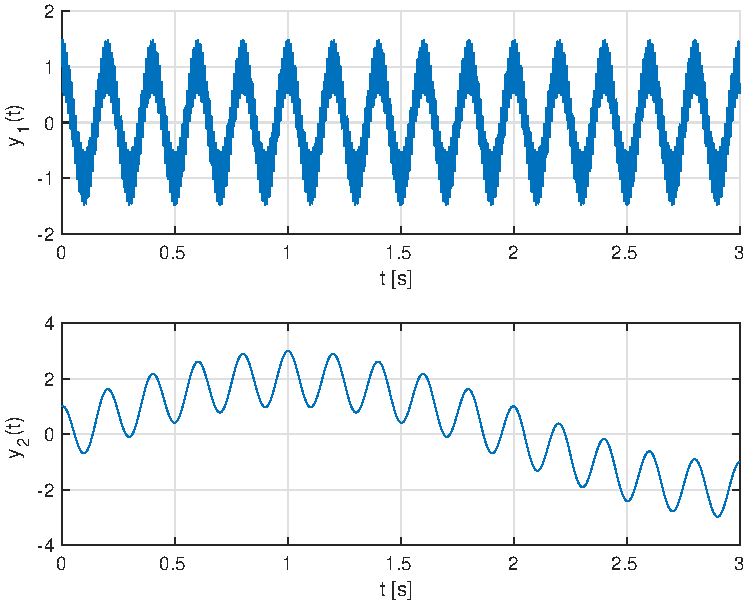
\includegraphics[width=\textwidth]{scf_meas.pdf}
    \caption{Measurements of $x(t)$.}
  \end{subfigure}
  \begin{subfigure}[t]{0.32\textwidth}
    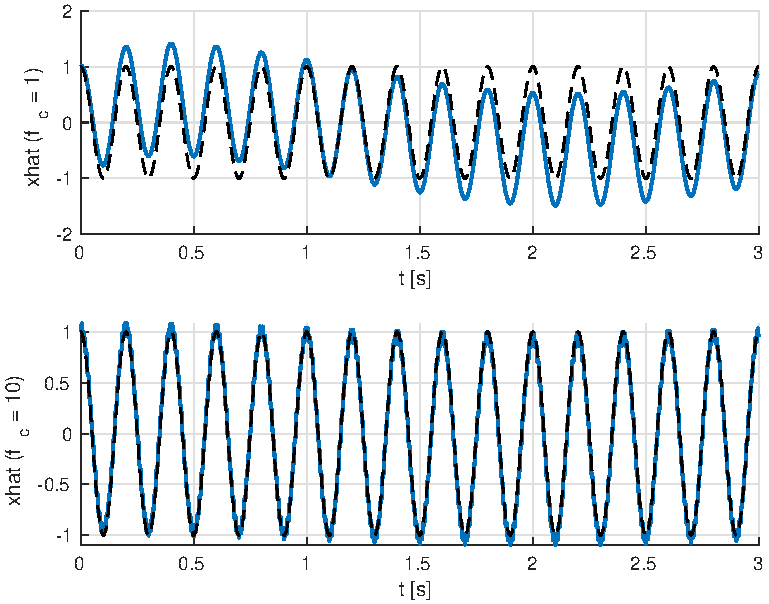
\includegraphics[width=\textwidth]{scf_est.pdf}
    \caption{Estimates using different $\omega_c$.}
  \end{subfigure}
  \begin{subfigure}[t]{0.32\textwidth}
    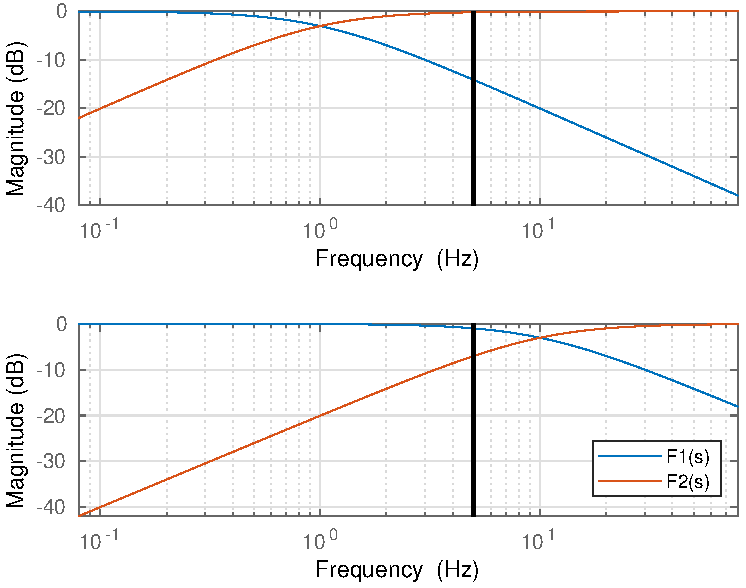
\includegraphics[width=\textwidth]{scf_bode.pdf}
    \caption{Bode magnitude plots of $F_1, F_2$ for different $\omega_c$.}
  \end{subfigure}
  \caption{Results from an example complementary filter.}
  \label{fig:scf}
\end{figure}

\section*{Mahony's Nonlinear Complementary Filter}
One of the more popular estimators is Mahony's nonlinear complementary filter on $\mathrm{SO}(3)$~\cite{Mahony2008}.

\begin{align}
  \dot{\bm{\hat{q}}} &= \frac{1}{2} \hat{\bm q} \otimes \bm{\bar \omega} \\
  \dot{\bm{\bar \omega}} &= (\bm{\omega} - \bm{b}) + k_P\bm{\omega}_\text{err} \\
  \dot{\bm{b}} &= -k_I\bm{\omega}_\text{err}
\end{align}

\begin{align}
  \bm{\omega}_\text{err} = \sum v_i \times \hat{v}_i
\end{align}

\begin{align}
  \tilde{\bm{q}} &= \hat{\bm q}^{-1} \otimes \bm{q}(\bm{a}) \\
  \bm{\omega}_\text{err} &= 2 q_w \bm{q}_\text{vec}
\end{align}

%%%%%%%%%%%%%%%%%%%%%%%%%%%%%%%%%%%%%%%%%%%%%%%%%%%%%%%%%%%%%%%%%%%%%%%%%%%%%%%
%%%%%%%%%%%%%%%%%%%%%%%%%%%%%%%%%%%%%%%%%%%%%%%%%%%%%%%%%%%%%%%%%%%%%%%%%%%%%%%
%%%%%%%%%%%%%%%%%%%%%%%%%%%%%%%%%%%%%%%%%%%%%%%%%%%%%%%%%%%%%%%%%%%%%%%%%%%%%%%
\bibliographystyle{IEEEtranN}
\bibliography{refs}

\end{document}
